\chapter{Entwicklung des Backends}\label{ch:Entwicklung des Backends}
\section{Entwurf der Architektur}\label{sec:Entwurf der Architektur}

\begin{wrapfigure}{r}{0.5\textwidth}
    \centering
    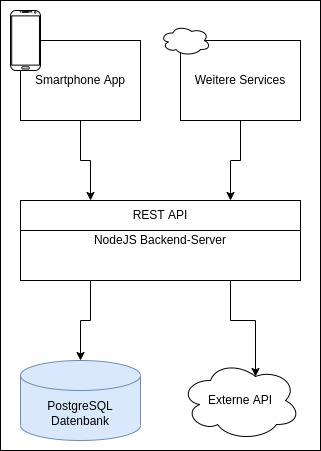
\includegraphics[width=0.5\textwidth]{figures/3.1.jpg}
    \caption{Architektur des \glsxtrshort{MVP}}
    \label{fig:3.1}
\end{wrapfigure}

Damit die zu entwickelnde Smartphone-App die Daten aus der Datenbank in aggregierter Form abrufen kann, wird eine zusätzliche Komponente benötigt. Der Backend-Server bildet wie in Abbildung~\ref{fig:3.1} dargestellt das Bindeglied zwischen Anwendungsprogrammen wie der Smartphone-App und der Datenbank. Darüber hinaus enthält das Backend die Verarbeitungslogik des Systems und reichert die Daten aus der Datenbank mit Daten aus externen Quellen an. Für die Entwicklung des Backends wird das Node.js-Framework NestJS verwendet.\\ Der Backend-Server bietet eine Schnittstelle in Form einer \gls{REST-API}, an die Anwendungen wie die Smartphone-App anknüpfen können. Der Backend-Server ist wie bei NestJS üblich in Module gegliedert die jeweils einer Tabelle im Datenbankmodell zugeordnet sind. Jedes Modul besteht dabei unter anderem aus einem Service, der die der jeweiligen Entitätsklasse zugehörige Verarbeitungslogik ausführt. Einigen Modulen sind zusätzlich mit Controllern ausgestattet. Ein Controller ist einer Route der API zugeordnet und bietet die Schnittstellenmethoden bzw. -operationen für diese an.

\FloatBarrier
\section{Implementierung des Datenbankmodells}\label{sec:Implementierung des Datenbankmodells}

Um die Kommunikation mit der Datenbank zu ermöglichen, hat jedes Modul Zugriff auf den Provider des Datenbank-Moduls. Darüber kann eine Verbindung zur Datenbank aufgebaut werden. Auch das Modell der jeweiligen Entitätsklasse ist zusätzlich jeweils in Form einer Klasse in der \textit{.entity.ts}-Datei des jeweiligen Moduls gespeichert. Die Klassen werden jeweils mit dem \textit{Table}-Dekorator des \glsxtrfull{ORM} Sequelize annotiert. Weitere Dekoratoren für die Definition von Domänen werden an den Attributen der Klassen angebracht. Beispielhaft ist die gekürzte Variante der Implementierung der Tabelle \textit{fridge\_user} im Codebeispiel~\ref{lst:3.1} zu sehen.\\

\lstinputlisting[caption=Sequelize-Entitätsklasse (gekürzte Darstellung), label=lst:3.1]{code/fridge_user.entity.ts}
